\documentclass[12pt]{exam}

% essential packages
\usepackage{fullpage} % margin formatting
\usepackage{enumitem} % configure enumerate and itemize
\usepackage{amsmath, amsfonts, amssymb, mathtools} % math symbols
\usepackage{xcolor, colortbl} % colors, including in tables
\usepackage{makecell} % thicker \Xhline in table
\usepackage{graphicx} % images, resizing
\usepackage{tikz} % drawing graphs
\usetikzlibrary{positioning}

% paragraph formatting
\setlength{\parskip}{6pt}
\setlength{\parindent}{0cm}

% newline after Solution:
\renewcommand{\solutiontitle}{\noindent\textbf{Solution:}\par\noindent}

% less space before itemize/enumerate
\setlist{topsep=0pt}

% creates \filcl to grey out cells for groupwork grading
\newcommand{\filcl}{\cellcolor{gray!25}}

% creates \probnum to get the problem number
\newcounter{probnumcount}
\setcounter{probnumcount}{1}
\newcommand{\probnum}{\arabic{probnumcount}. \addtocounter{probnumcount}{1}}

% use roman numerals by default
\setlist[enumerate]{label={(\roman*)}}

% creates custom list environments for grading guidelines, question parts
\newlist{guidelines}{itemize}{1}
\setlist[guidelines]{label={}, left=0pt .. \parindent, nosep}
\newlist{gwguidelines}{enumerate}{1}
\setlist[gwguidelines]{label={(\roman*)}, nosep}
\newlist{qparts}{enumerate}{2}
\setlist[qparts]{label={(\alph*)}}
\newlist{qsubparts}{enumerate}{2}
\setlist[qsubparts]{label={(\roman*)}}
\newlist{stmts}{enumerate}{1}
\setlist[stmts]{label={(\roman*)}, nosep}
\newlist{pflist}{itemize}{4}
\setlist[pflist]{label={$\bullet$}, nosep}
\newlist{enumpflist}{enumerate}{4}
\setlist[enumpflist]{label={(\arabic*)}, nosep}

\printanswers

\begin{document}
%%%%%%%%%%%%%%% TITLE PAGE %%%%%%%%%%%%%%%
\title{EECS 203: Discrete Mathematics\\
  Fall 2023\\
  Homework 10}
\date{}
\author{}
\maketitle
\vspace{-50pt}
\begin{center}
  \huge Due \textbf{Tuesday, November 28}, 10:00 pm\\
\Large No late homework accepted past midnight.\\
\vspace{10pt}
\large Number of Problems: $8+2$
\hspace{3cm}
Total Points: $100+30$
\end{center}
\vspace{25pt}
\begin{itemize}
    \item \textbf{Match your pages!} Your submission time is when you upload the file, so the time you take to match pages doesn't count against you.
    \item Submit this assignment (and any regrade requests later) on Gradescope. 
    \item Justify your answers and show your work (unless a question says otherwise).
    \item By submitting this homework, you agree that you are in compliance with the Engineering Honor Code and the Course Policies for 203, and that you are submitting your own work.
    \item Check the syllabus for full details.
\end{itemize}
\newpage
%%%%%%%%%%%%%%% TITLE PAGE %%%%%%%%%%%%%%% 


\section*{Individual Portion}


\textit{Reminder: }Make sure to leave your answers in combination, permutation, or factorial form and \textbf{not} simplified.

\subsection*{\probnum The Boxer and the Baller [12 points]}
How many ways are there to distribute seven balls into five boxes, where each box must have at least one ball in it, if
\begin{qparts}
    \item both the balls and boxes are unlabeled?

    \item the balls are labeled, but the boxes are unlabeled?
    \item both the balls and boxes are labeled?
\end{qparts}

\begin{solution}
    ~\\~\\~\\~\\~\\~\\~\\~\\~\\~\\~\\~\\~\\~\\~\\~\\~\\~\\~\\~\\~\\~\\
\end{solution}


\subsection*{\probnum Sweepstakes Sweep [12 points]}
Suppose that 100 people enter a contest and that different winners are selected at random for first, second, and third prizes. What is the probability that Kumar, Janice, and Pedro each win a prize if each has entered the contest?

\begin{solution}
    ~\\~\\~\\~\\~\\~\\~\\~\\~\\~\\~\\~\\~\\~\\~\\~\\~\\~\\~\\~\\~\\~\\
\end{solution}

\subsection*{\probnum Mississippi Bananas [8 points]}
How many different strings can be made by rearranging the letters in the word BANANANANAS?

\begin{solution}
    ~\\~\\~\\~\\~\\~\\~\\~\\~\\~\\~\\~\\~\\~\\~\\~\\~\\~\\~\\~\\~\\~\\
\end{solution}

\subsection*{\probnum Probabili-Tee [16 points]}
Tom has 30 T-shirts where 10 are blue, 5 are red, and 15 are green. Frank has 20 T-shirts where 13 are blue, 2 are red, and 5 are green. Both Tom and Frank own 1 green EECS 203 T-shirt, but only Tom owns 1 red and 1 blue EECS 203 T-shirt. Assume Frank and Tom pick and wear T-shirts uniformly at random. 

\begin{qparts}
    \item What is the probability that Tom and Frank are both wearing their green EECS 203 T-shirts, given that they're both wearing green T-shirts?

    \item What is the probability that Tom and Frank are both wearing a green T-shirt, given that they're both wearing the same type of T-shirt (both EECS 203 T-shirts or both not EECS 203 T-shirts)?
\end{qparts}

\begin{solution}
    ~\\~\\~\\~\\~\\~\\~\\~\\~\\~\\~\\~\\~\\~\\~\\~\\~\\~\\~\\~\\~\\~\\
\end{solution}


\subsection*{\probnum Independence Day [10 points]}

Let $E$ be the event that a randomly generated bit string of length three contains an odd number of 1s, and let $F$ be the event that the string starts with 1. Given that all bitstrings are equally likely to occur, are $E$ and $F$ independent?

\begin{solution}
    ~\\~\\~\\~\\~\\~\\~\\~\\~\\~\\~\\~\\~\\~\\~\\~\\~\\~\\~\\~\\~\\~\\
\end{solution}


\subsection*{\probnum $7+5=$ [12 points]}
Suppose we roll five fair \textbf{seven-sided} dice (there are seven faces, labeled 1 through 7). 

\begin{qparts}
    \item What is the probability that exactly four come up even? 
    \item What is the probability that exactly two come up even?
\end{qparts}

\begin{solution}
    ~\\~\\~\\~\\~\\~\\~\\~\\~\\~\\~\\~\\~\\~\\~\\~\\~\\~\\~\\~\\~\\~\\
\end{solution}


\subsection*{\probnum Driver's License [20 points]}
Suppose we're trying to come up with a new license plate system that must contain exactly 6 characters, each of which can be any of the following: an uppercase letter, lowercase letter, digit, or underscore character. How many possible license plate names are there given the following specifications? 
\begin{qparts}
    \item License plates cannot have a number character.
    \item License plates must have exactly one underscore character, which cannot be at the beginning or end of the license plate.
    \item License plates must have at least one number.
    \item License plates must have at least one number or at least one underscore character.
\end{qparts}
Justify your answer for each part.

\begin{solution}
    ~\\~\\~\\~\\~\\~\\~\\~\\~\\~\\~\\~\\~\\~\\~\\~\\~\\~\\~\\~\\~\\~\\~\\~\\~\\~\\~\\~\\~\\~\\~\\~\\~\\
\end{solution}


\subsection*{\probnum Pip Pip Hooray! [10 points]} 

One pip (small dot on the face of a die) is randomly removed from a standard eight-sided die (where its $8$ faces respectively have $\{1, 2, \dots, 8\}$ pips).
\textbf{Each pip} has an equal probability of being removed.
This means, for example, the face with 8 pips has a greater probability of losing a pip compared to the face with 1 pip.

What is the probability of rolling an even number on this die?

\begin{solution}
    ~\\~\\~\\~\\~\\~\\~\\~\\~\\~\\~\\~\\~\\~\\~\\~\\~\\~\\~\\~\\~\\~\\
\end{solution}

\pagebreak
\setcounter{probnumcount}{1}
\section*{Groupwork}
\subsection*{\probnum Grade Groupwork 9}
Using the solutions and Grading Guidelines, grade your Groupwork 9:
\begin{itemize}
    \item Mark up your past groupwork and submit it with this one.
    \item Write whether your submission achieved each rubric item. If it didn't achieve one, say why not.
    \item Use the table below to calculate scores.
    \item For extra credit, write positive comment(s) about your work.
    \item You don't have to redo problems correctly, but it is recommended!
    \item What if my group changed? \begin{itemize}
        \item If your current group submitted the same groupwork last time, grade it together.
        \item  If not, grade your version, which means submitting this groupwork assignment separately. You may discuss grading together.
    \end{itemize}
\end{itemize}

\begin{center}
\resizebox{\textwidth}{!}{\begin{tabular}{| c | c | c | c | c | c | c | c | c | c | c | c | c |}
\hline
 & (i) & (ii) & (iii) & (iv) & (v) & (vi) & (vii) & (viii) & (ix) & (x) & (xi) & Total:\\
\hline
Problem 2 & & & & & &\filcl &\filcl &\filcl &\filcl & \filcl& \filcl& \hspace{1cm}/15\\
\hline 
Problem 3 & & & & & & \filcl& \filcl &\filcl &\filcl & \filcl& \filcl& \hspace{1cm}/15\\
\Xhline{1.25pt}
Total: &\filcl &\filcl &\filcl &\filcl &\filcl &\filcl &\filcl &\filcl & \filcl& \filcl& \filcl&\hspace{1cm}/30\\
\hline
\end{tabular}}
\end{center}

\subsection*{Previous Groupwork 9(1): Square the Cycle [15 points]}
Prove that every $n$-node graph ($n \ge 3$) in which all nodes have degree at least $\lceil \sqrt{n} \rceil$ has a $3$-cycle subgraph or a $4$-cycle subgraph.

\textbf{Hint:} One useful concept is the neighborhood of a vertex; the neighborhood of $v\in V$ is the set $N(v)=\{u\in V : u\text{ is adjacent to }v\}.$ We can also define the neighborhood of a set $A\subseteq V$:
$$N(A)=\{u\in V : u\text{ is adjacent to some }v\in A\}.$$
We recommend using a proof by contradiction, although this can also be done with a clever direct proof. Suppose a graph satisfying the above condition does not have a 3-cycle or 4-cycle. Fix a vertex $v\in V.$ What can we say about the size of $N(v)$? What about $N(N(v))$?
\newpage

\begin{solution}
    ~\\~\\~\\~\\~\\~\\~\\~\\~\\~\\~\\~\\~\\~\\~\\~\\~\\~\\~\\~\\~\\~\\~\\~\\~\\~\\~\\~\\
\end{solution}

\subsection*{Previous Groupwork 9(2): The Office Allocation [15 points]}
Consider a new office building with $n$ floors and $k$ offices per floor in which you must assign $2nk$ people to work, each sharing an office with exactly one other person. Find a closed form solution for the number of ways there are to assign offices if from floor to floor the offices are distinguishable, but any two offices on a given floor are not.

\begin{solution}
    ~\\~\\~\\~\\~\\~\\~\\~\\~\\~\\~\\~\\~\\~\\~\\~\\~\\~\\~\\~\\~\\~\\~\\~\\~\\~\\~\\~\\
\end{solution}


\subsection*{\probnum Lily's Lily Pads [15 points]}
Lily the Frog is on a lily pad and wants to get to her home! She can jump from lily pad to lily pad to help reach this goal. The lily pads are arranged in a grid. Lily starts on the \textbf{bottom-left} lily pad, and her home is at the \textbf{top-right} lily pad. Lily can only move one lily pad \textbf{upward} or one lily pad \textbf{rightward} at a time.\\

Each lily pad has coordinates of the form $(x, y) \in \mathbb{N} \times \mathbb{N}$, where $x$ represents how far rightward a point is from the left of the grid, and $y$ represents how far upward a point is from the bottom of the grid. Lily starts at location $(0, 0)$, and her home is at location $(x_H, y_H)  \in \mathbb{N} \times \mathbb{N}$.\\

\begin{center}
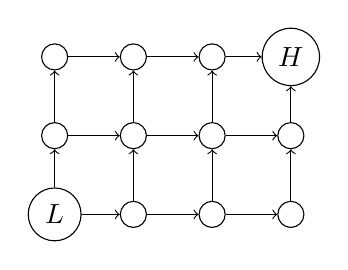
\begin{tikzpicture}[main/.style = {draw, circle}]
    \node[main] (1) {$L$};
    \node[main] (2) [above of=1] {};
    \node[main] (3) [above of=2] {};
    \node[main] (4) [right of=1] {};
    \node[main] (5) [above of=4] {};
    \node[main] (6) [above of=5] {};
    \node[main] (7) [right of=4] {};
    \node[main] (8) [above of=7] {};
    \node[main] (9) [above of=8] {};
    \node[main] (10) [right of=7] {};
    \node[main] (11) [above of=10] {};
    \node[main] (12) [above of=11] {$H$};
    \draw[->] (1) -- (2);
    \draw[->] (1) -- (4);
    \draw[->] (2) -- (3);
    \draw[->] (2) -- (5);
    \draw[->] (3) -- (6);
    \draw[->] (4) -- (5);
    \draw[->] (4) -- (7);
    \draw[->] (5) -- (6);
    \draw[->] (5) -- (8);
    \draw[->] (6) -- (9);
    \draw[->] (7) -- (8);
    \draw[->] (7) -- (10);
    \draw[->] (8) -- (9);
    \draw[->] (8) -- (11);
    \draw[->] (9) -- (12);
    \draw[->] (10) -- (11);
    \draw[->] (11) -- (12);
\end{tikzpicture}
\end{center}

In the above example, $(x_H, y_H) = (3, 2)$. In the general case, though, $(x_H, y_H)$ could be any ordered pair of natural numbers.

\begin{qparts}
    \item How many different paths can Lily take to get home?
    \item Lily's frog friend, Francine, is also on the grid at coordinates $(x_F, y_F) \in \mathbb{N} \times \mathbb{N}$ such that $0 \leq x_F \leq x_H$ and $0 \leq y_F \leq y_H$. What is the probability that Lily meets Francine on her path home? You may assume that any two paths home are equally likely for Lily to take.
\end{qparts}
\begin{solution}
    ~\\~\\~\\~\\~\\~\\~\\~\\~\\~\\~\\~\\~\\~\\~\\~\\~\\~\\~\\~\\~\\~\\~\\~\\~\\~\\~\\~\\
    ~\\~\\~\\~\\~\\~\\~\\~\\~\\~\\~\\~\\~\\~\\~\\
\end{solution}

\subsection*{\probnum Random Connections [15 points]}
We say that a \textit{random graph} is an undirected graph where, for each pair of vertices, there is an independent $\frac{1}{3}$ chance that they are adjacent. It's a bit like Lily's pond, except that the vertices aren't in a grid, and you can move in any direction.

We want to learn about the connectedness of random graphs.

Let $G$ be a finite random graph. Let's split the vertices into two nonempty sets, $A, B \subseteq V$.

\begin{qparts}
    \item Let $a \in A$. What is the probability that no element of $B$ is adjacent to $a$?
    \item What is the probability that there is some $a \in A$ and $b \in B$ such that $a$ is adjacent to $b$?
    \item Let's imagine doing this with larger and larger graphs. Define $f(a, b)$ be your answer to the previous problem when $|A| = a$ and $|B| = b$. What is
    \[ \lim_{a+b \to \infty} f(a,b)? \]
    \item This isn't quite a proof, but your answer to (c) might lead you to some ideas. What might you conjecture about the connectedness of infinite random graphs?
\end{qparts}
\begin{solution}
    ~\\~\\~\\~\\~\\~\\~\\~\\~\\~\\~\\~\\~\\~\\~\\~\\~\\~\\~\\~\\~\\~\\~\\~\\~\\~\\~\\~\\
    ~\\~\\~\\~\\~\\~\\~\\~\\
\end{solution}

\end{document}
